\documentclass[11pt,a4paper]{article}
\usepackage{fontspec}
\setmainfont{CMU Serif}
\setsansfont{CMU Sans Serif}
\setmonofont{CMU Typewriter Text}
\usepackage[a4paper,left=2.2cm,right=2.2cm,top=2.2cm,bottom=2.4cm]{geometry}
\usepackage{amssymb}
\usepackage{pgfplots,subcaption,fancyvrb}
\usepackage[most]{tcolorbox}
\usetikzlibrary{decorations.pathreplacing,shapes.geometric}
\usepackage{xcolor,graphicx,tabularx,booktabs,colortbl,longtable,array,enumitem,caption,titlesec,fancyhdr,listings,amsmath,tikz,float}
\usetikzlibrary{positioning,arrows.meta}
\usepackage[hidelinks]{hyperref}
\definecolor{navy}{HTML}{1F3864}
\definecolor{hblue}{HTML}{2E75B6}
\definecolor{codebg}{HTML}{F6F7F9}
\definecolor{fillc}{HTML}{C55A11}
\definecolor{notebg}{HTML}{FFF8E1}
\definecolor{grn}{HTML}{22A06B}\definecolor{rd}{HTML}{D9534F}\definecolor{yl}{HTML}{E0A100}
\setlength{\parindent}{0pt}\setlength{\parskip}{5pt}
\sloppy
\titleformat{\section}{\sffamily\Large\color{navy}}{\thesection.}{0.5em}{}
\titleformat{\subsection}{\sffamily\large\color{hblue}}{\thesubsection}{0.6em}{}
\titleformat{\subsubsection}{\sffamily\normalsize\bfseries\color{navy}}{}{0em}{}
\titlespacing*{\section}{0pt}{14pt}{6pt}
\titlespacing*{\subsection}{0pt}{10pt}{4pt}
\captionsetup{font=small,labelfont=it,textfont=it,labelsep=period}
\setlist{itemsep=1pt,topsep=2pt}
\newcolumntype{Y}{>{\raggedright\arraybackslash}X}
\newcommand{\hc}[1]{\textcolor{white}{\textbf{#1}}}
\newcommand{\hdr}{\rowcolor{navy}}
\newcommand{\fillin}[1]{\textcolor{fillc}{\textit{#1}}}
\renewcommand{\arraystretch}{1.18}
\lstset{basicstyle=\ttfamily\small,backgroundcolor=\color{codebg},frame=single,rulecolor=\color{black!25},
  breaklines=true,columns=fullflexible,keepspaces=true,xleftmargin=4pt,xrightmargin=4pt,aboveskip=6pt,belowskip=6pt,
  extendedchars=true,showstringspaces=false}
\newcommand{\notebox}[1]{\par\noindent\colorbox{notebg}{\parbox{\dimexpr\linewidth-2\fboxsep}{\small #1}}\par}
\pagestyle{fancy}\fancyhf{}
\renewcommand{\headrulewidth}{0pt}
\fancyfoot[R]{\small\thepage}
\newcommand{\coverpage}[1]{%
\begin{titlepage}\centering
{\large\textsc{Шинжлэх Ухаан Технологийн Их Сургууль}\par}\vspace{2pt}
{\textsc{Мэдээлэл, Холбооны Технологийн Сургууль}\par}
\vspace{1cm}
\includegraphics[height=3.6cm]{logo.png}\par\vspace{1.8cm}
{\large F.CSM302\quad Үйлдлийн систем\par}
\vspace{2.2cm}{\Large Бие даалт №1\par}\vspace{8pt}{\LARGE\textbf{#1}\par}\vspace{6pt}{\color{hblue}\rule{0.55\linewidth}{0.8pt}}\par
\vspace{0.2cm}{\normalsize Хуваарилалтын код: II-4-15\par}
\vspace{2.6cm}
\begin{tabular}{@{}p{5.6cm}l@{}}
\textit{Шалгасан багш:} & Г.Ганбат /F.CS10/\\[2pt]
\textit{Гүйцэтгэсэн оюутан:} & Э.Мөнх-Оргил /B242270130/\\
 & Д.Ундармаа /B242270044/\\
 & В.Хүсэлбилэг /B241910007/\\
 & С.Сүхбат /B241940044/\\
 & М.Хатансайхан /B231940049/\\
\end{tabular}
\vfill
Улаанбаатар хот\par 2026 он
\end{titlepage}}
\setlength{\emergencystretch}{3em}
\renewcommand{\figurename}{Зураг}\renewcommand{\tablename}{Хүснэгт}
\renewcommand{\contentsname}{Агуулга}
\graphicspath{{../img/}}
\newenvironment{term}{\VerbatimEnvironment\begin{tcolorbox}[colback=codebg,colframe=black!25,boxrule=0.4pt,arc=0pt,left=3pt,right=3pt,top=2pt,bottom=2pt]\begin{Verbatim}[fontsize=\footnotesize]}{\end{Verbatim}\end{tcolorbox}}

\fancyfoot[L]{\small\color{black!55}II-4-15 · Virtual Memory Manager · F.CSM302 Бие даалт 1 · Тайлан}
% ---- pgfplots style ----
\definecolor{cfifo}{HTML}{2A78D6}\definecolor{clru}{HTML}{EB6834}
\pgfplotsset{compat=1.18,
  every axis/.append style={font=\footnotesize, axis lines=left, grid=major, major grid style={black!10},
    title style={font=\small\sffamily\color{navy}}, legend style={draw=none, fill=white, fill opacity=0.85, text opacity=1, font=\footnotesize},
    tick align=outside, axis line style={black!45}},
  fifo/.style={cfifo, line width=1.4pt, mark=*, mark size=2pt, mark options={fill=white, line width=1pt}},
  lru/.style={clru, line width=1.4pt, mark=square*, mark size=2pt, mark options={fill=white, line width=1pt}}}
\newcommand{\plotLocality}[1][0.48\linewidth]{%
\begin{tikzpicture}\begin{axis}[width=#1, height=0.62*#1, xmode=log, log basis x=2, xtick={8,16,32,64,128,256}, xticklabels={8,16,32,64,128,256},
 title={Locality өгөгдөл (1000 хаяг)}, xlabel={Frame-ийн тоо}, ylabel={Page fault rate, \%}, ymin=10,ymax=52]
\addplot[fifo] coordinates {(8,47.8) (16,27.7) (32,21.4) (64,19.3) (128,16.6) (256,16.1)}; \addlegendentry{FIFO}
\addplot[lru] coordinates {(8,44.5) (16,22.6) (32,21.0) (64,19.2) (128,16.6) (256,16.1)}; \addlegendentry{LRU}
\end{axis}\end{tikzpicture}}
\newcommand{\plotBook}[1][0.48\linewidth]{%
\begin{tikzpicture}\begin{axis}[width=#1, height=0.62*#1, xmode=log, log basis x=2, xtick={8,16,32,64,128,256}, xticklabels={8,16,32,64,128,256},
 title={Номын addresses.txt (1000 хаяг)}, xlabel={Frame-ийн тоо}, ylabel={Page fault rate, \%}, ymin=20,ymax=100]
\addplot[fifo] coordinates {(8,97.5) (16,94.6) (32,88.2) (64,76.2) (128,53.8) (256,24.4)}; \addlegendentry{FIFO}
\addplot[lru] coordinates {(8,97.5) (16,94.5) (32,87.9) (64,75.4) (128,53.9) (256,24.4)}; \addlegendentry{LRU}
\node[font=\scriptsize, navy, anchor=north east, align=right] at (axis cs:256,40) {256 frame: 244 fault\\= ялгаатай page-ийн тоо};
\end{axis}\end{tikzpicture}}
\newcommand{\plotTLB}[1][0.48\linewidth]{%
\begin{tikzpicture}\begin{axis}[width=#1, height=0.62*#1, xmode=log, log basis x=2, xtick={1,2,4,8,16,32,64}, xticklabels={1,2,4,8,16,32,64},
 title={TLB hit rate (locality, 256 frame)}, xlabel={TLB-ийн хэмжээ}, ylabel={TLB hit rate, \%}, ymin=0,ymax=90,legend pos=south east]
\addplot[fifo] coordinates {(1,9.8) (2,18.5) (4,31.9) (8,52.2) (16,72.3) (32,78.6) (64,80.7)}; \addlegendentry{FIFO}
\addplot[lru] coordinates {(1,9.8) (2,18.2) (4,33.2) (8,55.5) (16,77.4) (32,79.0) (64,80.8)}; \addlegendentry{LRU}
\end{axis}\end{tikzpicture}}
\newcommand{\plotBelady}[1][0.48\linewidth]{%
\begin{tikzpicture}\begin{axis}[width=#1, height=0.62*#1, xtick={1,2,3,4,5,6}, xticklabels={1,2,3,4,5,6},
 title={Belady: 1 2 3 4 1 2 5 1 2 3 4 5}, xlabel={Frame-ийн тоо}, ylabel={Page fault}, ymin=0,ymax=13,legend pos=south west]
\addplot[fifo] coordinates {(1,12) (2,12) (3,9) (4,10) (5,5) (6,5)}; \addlegendentry{FIFO}
\addplot[lru] coordinates {(1,12) (2,12) (3,10) (4,8) (5,5) (6,5)}; \addlegendentry{LRU}
\draw[navy, line width=0.6pt] (axis cs:4,10) circle (5pt);
\node[font=\scriptsize, navy, anchor=south west, align=left] at (axis cs:4.15,10.4) {FIFO: 3→4 frame үед\\fault 9→10 өссөн};
\end{axis}\end{tikzpicture}}


% ---- Гол үр дүнгийн хайрцаг ----
\newcommand{\stat}[2]{\begin{minipage}[t]{0.235\linewidth}\centering{\sffamily\LARGE\color{navy}\textbf{#1}}\\[2pt]{\footnotesize #2}\end{minipage}}
\newcommand{\keyresults}{%
\begin{tcolorbox}[colback=hblue!6, colframe=hblue!60, boxrule=0.6pt, arc=2pt, left=4pt, right=4pt, top=6pt, bottom=6pt,
  title={\sffamily Гол үр дүн}, coltitle=white, colbacktitle=navy, fonttitle=\small]
\stat{1000/1000}{Номын correct.txt-тэй\\таарсан мөр (256 frame)}\hfill
\stat{15 / 12}{Номын жишээ: FIFO / LRU\\fault (номтой таарсан)}\hfill
\stat{9 → 10}{Belady-ийн аномали\\(FIFO, 3 → 4 frame)}\hfill
\stat{22.6\%}{LRU fault rate (16 frame)\\FIFO-д 27.7\%}
\end{tcolorbox}}

% ---- Хаяг задлах диаграм (16916) ----
\newcommand{\addrsplit}{%
\begin{tikzpicture}[font=\footnotesize, bit/.style={draw=black!50, minimum width=6.2mm, minimum height=7mm, inner sep=0pt, font=\ttfamily}]
\node[anchor=east, font=\small] at (-0.15,0.35) {16916 =};
\foreach \b [count=\i from 0] in {0,1,0,0,0,0,1,0}
  \node[bit, fill=hblue!25, anchor=south west] at (\i*0.62,0) {\b};
\foreach \b [count=\i from 8] in {0,0,0,1,0,1,0,0}
  \node[bit, fill=clru!22, anchor=south west] at (\i*0.62,0) {\b};
\draw[decorate, decoration={brace, amplitude=5pt, mirror}, thick, navy] (0,-0.08) -- (4.96,-0.08)
  node[midway, below=6pt, align=center] {\textbf{page} = 0100 0010$_2$ = \textbf{66}\\(дээд 8 бит: \texttt{a >> 8})};
\draw[decorate, decoration={brace, amplitude=5pt, mirror}, thick, clru!80!black] (4.96,-0.08) -- (9.92,-0.08)
  node[midway, below=6pt, align=center] {\textbf{offset} = 0001 0100$_2$ = \textbf{20}\\(доод 8 бит: \texttt{a \& 0xFF})};
\node[anchor=west, align=left, font=\small] at (10.3,0.35) {page 66 → frame 0\\физик = 0×256 + 20 = \textbf{20}};
\node[font=\scriptsize, black!60] at (0.31,0.95) {15}; \node[font=\scriptsize, black!60] at (9.61,0.95) {0};
\end{tikzpicture}}

% ---- Хаяг хөрвүүлэх урсгал ----
\newcommand{\translationflow}{%
\begin{tikzpicture}[font=\footnotesize, >={Stealth[length=2mm]},
  b/.style={draw=navy, rounded corners=2pt, fill=hblue!8, align=center, inner sep=4pt, minimum height=9mm},
  d/.style={draw=navy, diamond, aspect=2.2, fill=white, align=center, inner sep=1pt},
  lab/.style={font=\scriptsize\itshape, black!70}]
\node[b] (cpu) at (0,0) {Логик хаяг\\\texttt{page | offset}};
\node[d] (tlb) at (3.6,0) {TLB-д\\байна уу?};
\node[d] (pt) at (3.6,-2.3) {page\_table\\$\neq -1$?};
\node[b, fill=rd!12, draw=rd] (pf) at (3.6,-4.4) {\textbf{Page fault}\\хоосон frame эсвэл\\FIFO/LRU victim};
\node[b] (bs) at (-0.9,-4.4) {Backing store\\(256 байт уншина)};
\node[b] (upd) at (7.6,-3.3) {page\_table ба TLB-г\\шинэчилнэ (victim-ийг\\хүчингүй болгоно)};
\node[b, fill=grn!12, draw=grn] (fr) at (7.6,0) {\textbf{frame}};
\node[b] (pa) at (11.2,0) {Физик хаяг\\frame×256 + offset};
\draw[->] (cpu)--(tlb);
\draw[->, grn!70!black, thick] (tlb)--node[above, lab]{hit}(fr);
\draw[->] (tlb)--node[right, lab]{miss}(pt);
\draw[->] (pt.east) -| node[pos=0.25, above, lab]{тийм} ([xshift=-6mm]fr.south);
\draw[->, rd] (pt)--node[right, lab]{үгүй}(pf);
\draw[->, dashed] (bs)--node[above, lab]{ачаална}(pf);
\draw[->] (pf.east) -| (upd.south);
\draw[->] (upd)--(fr);
\draw[->] (fr)--(pa);
\end{tikzpicture}}

% ---- Дугаартай тайлбартай GUI ----
\newcommand{\callout}[3]{\node[circle, fill=rd, text=white, font=\footnotesize\bfseries\sffamily, inner sep=1.2pt, minimum size=4.6mm, draw=white, line width=0.8pt] at (#1,#2) {#3};}
\newcommand{\annotatedgui}{%
\begin{tikzpicture}
\node[anchor=south west, inner sep=0] (img) at (0,0) {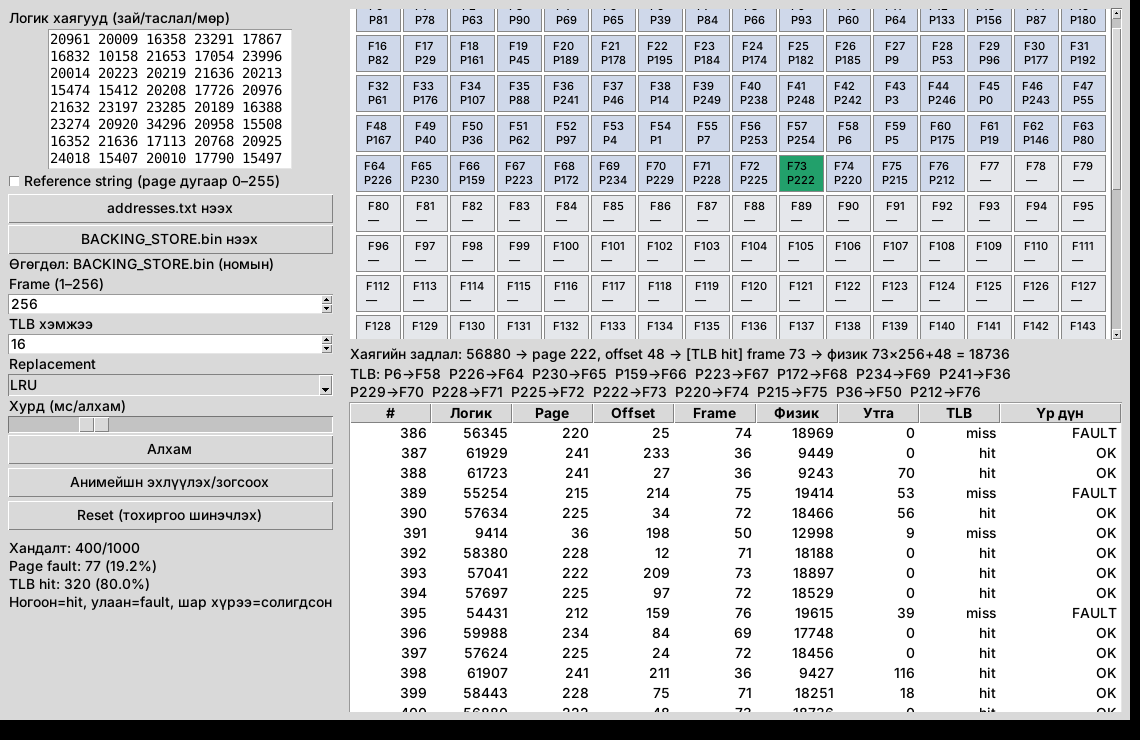
\includegraphics[width=0.93\linewidth]{gui_big.png}};
\begin{scope}[x={(img.south east)}, y={(img.north west)}]
\callout{-0.022}{0.88}{1} \callout{-0.022}{0.62}{2} \callout{-0.022}{0.35}{3} \callout{-0.022}{0.21}{4}
\callout{0.33}{0.96}{5} \callout{0.975}{0.523}{6} \callout{0.975}{0.478}{7} \callout{0.33}{0.40}{8}
\end{scope}
\end{tikzpicture}}

\hypersetup{pdftitle={II-4-15 Designing a Virtual Memory Manager — Бие даалт 1 тайлан},
  pdfauthor={Э.Мөнх-Оргил, Д.Ундармаа, В.Хүсэлбилэг, С.Сүхбат, М.Хатансайхан},
  pdfsubject={F.CSM302 Үйлдлийн систем, Бие даалт 1}, pdfkeywords={virtual memory, TLB, page table, FIFO, LRU}}
\setcounter{tocdepth}{2}
\begin{document}
\coverpage{Designing a Virtual Memory Manager}
{\setlength{\parskip}{1pt}\tableofcontents}
\clearpage

% ---------------------------------------------------------------
\section*{Хураангуй}\addcontentsline{toc}{section}{Хураангуй}
\textbf{Асуудал.} Сурах бичгийн 10-р бүлгийн Programming Project нь виртуал санах ойн менежер бичихийг шаарддаг. Програм нь 32 битийн логик хаягийн баруун 16 битийг 8 битийн page дугаар, 8 битийн offset болгон задалж, TLB болон page table ашиглан физик хаяг руу хөрвүүлнэ. Page fault гарвал backing store-оос page ачаалж, санах ой дүүрсэн үед page солино.

\textbf{Шийдэл.} Python 3 хэл дээр физик санах ойг бүрэн загварчилсан \texttt{vmm.py} цөм модуль хөгжүүлэв. Түүнийг ашигладаг номын гаралттай ижил форматтай консол програм (\texttt{cli.py}), FIFO/LRU-г харьцуулах туршилтын скрипт (\texttt{experiment.py}), tkinter-ийн \textbf{page/frame animation} бүхий interactive UI (\texttt{gui.py}) бичсэн. Хэрэглэгч хаяг эсвэл reference string, frame-ийн тоо (1–256), TLB-ийн хэмжээ, replacement бодлого, backing store файлыг сольж дахин туршиж болно.

\textbf{Туршилт.} Сурах бичгийн албан ёсны \texttt{addresses.txt}, \texttt{BACKING\_STORE.bin}, \texttt{correct.txt} файлууд дээр туршив. Үүнээс гадна номын хоёр reference string, locality-тэй 1000 хаяг, захын болон алдаатай оролт, 24 автомат тест ашиглав.

\textbf{Гол үр дүн.} Номын 1000 хаягийг 256 frame-тэй хөрвүүлэхэд гаралт \texttt{correct.txt}-тэй \textbf{1000/1000 мөр яг таарав} (Page Faults = 244, TLB Hits = 54). 128 frame-тэй үед FIFO 538, LRU 539 fault гарсан бөгөөд 1000 утга бүгд зөв хэвээр байлаа. Номын reference string дээр 3 frame-тэй үед \textbf{FIFO 15, LRU 12} fault гарч номын хариутай таарав. Belady-ийн аномали ч давтагдсан. Locality-тэй өгөгдөлд 16 frame үед LRU 22.6\%, FIFO 27.7\% fault rate гарсан. Харин санамсаргүй хаягтай номын өгөгдөлд хоёр алгоритмын ялгаа бараг байсангүй.

\keyresults

\textbf{Хязгаарлалт (товч).} Ном шаардаагүй тул бичих үйлдэл (dirty bit) болон олон процесс хэрэгжээгүй. TLB нь page replacement-тэй ижил бодлогоор солигддог.

% ---------------------------------------------------------------
\section{Удиртгал}
\subsection{Зорилго}
Виртуал санах ойн хаяг хөрвүүлэлт (address translation), TLB, demand paging болон page replacement алгоритмыг өөрсдөө хэрэгжүүлнэ. Хэрэгжүүлсэн програмаа номын албан ёсны өгөгдлөөр баталгаажуулж, ажиллагааг нь алхам алхмаар дүрслэн харуулна. Мөн параметр өөрчлөхөд гүйцэтгэл хэрхэн өөрчлөгдөхийг туршилтаар нотолно.
\subsection{Ач холбогдол}
Орчин үеийн ихэнх үйлдлийн систем paging-д суурилсан виртуал санах ой ашигладаг. Лекц дээр онолоор үзсэн page table, TLB, page fault, FIFO/LRU, Belady-ийн аномали зэрэг ойлголтыг ажиллаж буй програм дээр харж, тоон үр дүнгээр баталгаажуулах нь ойлголтыг гүнзгийрүүлнэ.
\subsection{Хамрах хүрээ}
$2^{16}=65\,536$ байт виртуал хаягийн орон зай, 256 байтын page, 256 page, 1–256 frame, дурын хэмжээтэй TLB, FIFO ба LRU бодлого. Бичих үйлдэл (dirty page), олон процесс, олон түвшний page table хамрах хүрээнд ороогүй. Эдгээрийг ном ч шаардаагүй.

% ---------------------------------------------------------------
\section{Сурах бичгийн шаардлага}
Сурах бичгийн 10-р бүлгийн „Designing a Virtual Memory Manager“ төслийн үндсэн шаардлага ба тэдгээрийн хэрэгжилт:

\begin{tabularx}{\linewidth}{@{}c>{\raggedright\arraybackslash}p{5.3cm}Yl@{}}
\hdr\hc{№}&\hc{Шаардлага}&\hc{Хэрэгжилт}&\hc{Төлөв}\\
1&Баруун 16 битийг 8 битийн page, 8 битийн offset болгон задлах&\texttt{a = addr \& 0xFFFF; page = a >> 8; offset = a \& 0xFF}&Хэрэгжсэн\\
2&$2^8$ page table оролт, $2^8$ байт page/frame, 256 frame (65\,536 байт физик санах ой)&\texttt{PAGE\_SIZE = NUM\_PAGES = MAX\_FRAMES = 256}, \texttt{memory = bytearray(frames*256)}&Хэрэгжсэн\\
3&16 оролттой TLB. TLB miss үед page table&\texttt{VMM(tlb\_size=16)}. TLB → page table дараалал&Хэрэгжсэн\\
4&Page fault үед \texttt{BACKING\_STORE.bin}-оос 256 байт уншиж, хоосон frame-д хадгалах (demand paging)&\texttt{memory[frame*256 ...] = store[page*256 ...]}&Хэрэгжсэн\\
5&Физик санах ой дахь signed byte утгыг гаргах&\texttt{b - 256 if b > 127 else b}&Хэрэгжсэн\\
6&Гаралт: логик хаяг, физик хаяг, утга. Page-fault rate, TLB hit rate&\texttt{cli.py} номын форматаар&Хэрэгжсэн\\
7&Гаралтыг \texttt{correct.txt}-ээр шалгах&\texttt{tools/check\_correct.py}: 1000/1000&Хэрэгжсэн\\
8&Өөрчлөлт: 128 frame, page replacement (FIFO эсвэл LRU)&\texttt{--frames 1..256 --policy FIFO|LRU}&Хэрэгжсэн\\
9&TLB-ийн солих бодлого (FIFO эсвэл LRU)&TLB сонгосон бодлогоор солигдоно&Хэрэгжсэн\\
\end{tabularx}

Багшийн хуваарилалтад заасан нэмэлт шаардлага: \textit{„Address эсвэл reference sequence, frame-ийн тоо, replacement сонголтыг өөрчилж, page/frame-ийн өөрчлөлт, hit, fault-ийг алхамчилж харуулна.“} Энэ шаардлагыг GUI-ийн reference string горим, frame/TLB/policy тохиргоо, Алхам ба Анимейшн товчоор хангасан.

% ---------------------------------------------------------------
\section{Онолын үндэс}
\subsection{Виртуал санах ой ба paging}
Процесс бүр өөрийн логик хаягийн орон зайтай. Үйлдлийн систем түүнийг ижил хэмжээтэй \textit{page}-д хувааж, физик санах ойн \textit{frame}-д байрлуулна. Page table нь page дугаарыг frame дугаар руу буулгадаг. Санах ой руу хандах бүрт page table руу давхар хандахгүйн тулд сүүлийн хөрвүүлэлтүүдийг \textit{TLB} хэмээх жижиг, хурдан кэшэд хадгална.

\begin{tabularx}{\linewidth}{@{}>{\raggedright\arraybackslash}p{2.9cm}YY@{}}
\hdr\hc{Нэр томьёо}&\hc{English}&\hc{Монгол}\\
Page / Frame&Fixed-size block of virtual / physical memory&Виртуал / физик санах ойн тогтмол хэмжээтэй хэсэг (энд 256 байт)\\
Page table&Maps page number → frame number&Page бүр аль frame-д байгааг заасан хүснэгт\\
TLB&Small fast cache of recent page→frame translations&Сүүлийн хөрвүүлэлтүүдийг хадгалах хурдан кэш\\
Page fault&Trap when a referenced page is not in memory&Хандсан page санах ойд байхгүй үед үүсэх тасалдал\\
Demand paging&Load a page only when first referenced&Page-ийг анх хандах үед нь л ачаалах\\
Backing store&Secondary storage holding all pages&Бүх page хадгалагддаг хоёрдогч санах ой (энд \texttt{BACKING\_STORE.bin})\\
FIFO&Replace the page loaded earliest&Хамгийн эрт ачаалсан page-ийг солих\\
LRU&Replace the page unused for the longest time&Хамгийн удаан хэрэглээгүй page-ийг солих\\
Belady's anomaly&More frames can cause more faults (FIFO)&Frame нэмэхэд fault өсөх үзэгдэл\\
Locality&Programs reuse a small working set for a while&Програм тодорхой хугацаанд цөөн page-д давтан хандах шинж\\
\end{tabularx}

\subsection{Өгөгдлийн бүтэц}
\begin{tabularx}{\linewidth}{@{}llY@{}}
\hdr\hc{Нэр}&\hc{Хэмжээс}&\hc{Утга}\\
\textbf{page\_table}&256&Page бүрийн frame дугаар, санах ойд байхгүй бол $-1$\\
\textbf{memory}&$F\times256$&Физик санах ой (\texttt{bytearray}). Frame $f$ нь $[f\cdot256,\ (f+1)\cdot256)$ байт\\
\textbf{frames}&$F\times3$&Frame бүрийн \texttt{[page, loaded, used]}. \texttt{loaded}: ачаалсан цаг, \texttt{used}: сүүлд хандсан цаг\\
\textbf{tlb}&$\le T$&\texttt{[page, frame, loaded, used]} оролтууд\\
\textbf{clock}&1&Хандалт бүрт 1-ээр өсөх логик цаг\\
\textbf{store}&65\,536&Backing store (\texttt{BACKING\_STORE.bin} эсвэл жишиг өгөгдөл)\\
\end{tabularx}

\subsection{Хаяг хөрвүүлэх алгоритм}
Жишээ болгон номын эхний хаяг 16916-г авч үзье. Баруун 16 битийг хоёр 8 битэд хуваана:
\begin{figure}[H]\centering\resizebox{\linewidth}{!}{\addrsplit}
\caption{16 битийн логик хаягийг page ба offset болгон задлах (16916 → page 66, offset 20)}\end{figure}
Ерөнхий алгоритм:
\begin{enumerate}
\item $a = \text{addr} \mathbin{\&} \text{0xFFFF}$, \ $\text{page} = a \gg 8$, \ $\text{offset} = a \mathbin{\&} \text{0xFF}$
\item TLB-ээс page-ийг хайна. Олдвол frame-ийг авна → \textbf{TLB hit}
\item Олдохгүй бол $\text{page\_table}[\text{page}]$-ийг шалгана. $\ge 0$ бол frame-ийг авна
\item $-1$ бол \textbf{PAGE FAULT}: хоосон frame байвал түүнийг авна, үгүй бол FIFO/LRU-гаар victim сонгож, түүний page table ба TLB оролтыг хүчингүй болгоно. Дараа нь backing store-оос 256 байтыг тэр frame руу хуулна
\item TLB-д $(\text{page},\text{frame})$-ийг нэмнэ. TLB дүүрсэн бол FIFO/LRU-гаар нэг оролтыг гаргана
\item $\text{physical} = \text{frame}\times256 + \text{offset}$, \ $\text{value} = \text{signed}(\text{memory}[\text{physical}])$
\end{enumerate}
\begin{figure}[H]\centering\resizebox{\linewidth}{!}{\translationflow}
\caption{Хаяг хөрвүүлэх урсгал: TLB → page table → page fault}\end{figure}
Хандалт бүрийн хугацааны нарийвчлал нь TLB хайлтад $O(T)$, victim сонголтод $O(F)$ байна.

\subsection{Page replacement: FIFO ба LRU}
FIFO нь \texttt{loaded}-ийн хамгийн бага утгатай frame-ийг, LRU нь \texttt{used}-ийн хамгийн бага утгатай frame-ийг victim болгоно. LRU нь \textit{stack алгоритм} тул $n$ frame-д байгаа page-ийн олонлог нь $n+1$ frame-ийнхийн дэд олонлог байдаг. Иймээс frame нэмэхэд fault хэзээ ч өсдөггүй. FIFO-д энэ шинж байхгүй тул Belady-ийн аномали гарч болно.

\subsection{Гараар бодсон сурах бичгийн жишээ}
Reference string \texttt{7 0 1 2 0 3 0 4 2 3 0 3 2 1 2 0 1 7 0 1}, 3 frame. Багана нь F0, F1, F2 frame-ийн агуулга. \textbf{F} нь page fault, ($-p$) нь гаргасан page:

{\small
\begin{longtable}{@{}cc|lc|lc@{}}
\hdr\hc{\#}&\hc{Page}&\hc{FIFO: F0 F1 F2}&\hc{Үр дүн}&\hc{LRU: F0 F1 F2}&\hc{Үр дүн}\\
\endhead
1 & 7 & 7 -- -- & \textbf{F} & 7 -- -- & \textbf{F} \\
2 & 0 & 7 0 -- & \textbf{F} & 7 0 -- & \textbf{F} \\
3 & 1 & 7 0 1 & \textbf{F} & 7 0 1 & \textbf{F} \\
4 & 2 & 2 0 1 & \textbf{F} ($-$7) & 2 0 1 & \textbf{F} ($-$7) \\
5 & 0 & 2 0 1 & hit & 2 0 1 & hit \\
6 & 3 & 2 3 1 & \textbf{F} ($-$0) & 2 0 3 & \textbf{F} ($-$1) \\
7 & 0 & 2 3 0 & \textbf{F} ($-$1) & 2 0 3 & hit \\
8 & 4 & 4 3 0 & \textbf{F} ($-$2) & 4 0 3 & \textbf{F} ($-$2) \\
9 & 2 & 4 2 0 & \textbf{F} ($-$3) & 4 0 2 & \textbf{F} ($-$3) \\
10 & 3 & 4 2 3 & \textbf{F} ($-$0) & 4 3 2 & \textbf{F} ($-$0) \\
11 & 0 & 0 2 3 & \textbf{F} ($-$4) & 0 3 2 & \textbf{F} ($-$4) \\
12 & 3 & 0 2 3 & hit & 0 3 2 & hit \\
13 & 2 & 0 2 3 & hit & 0 3 2 & hit \\
14 & 1 & 0 1 3 & \textbf{F} ($-$2) & 1 3 2 & \textbf{F} ($-$0) \\
15 & 2 & 0 1 2 & \textbf{F} ($-$3) & 1 3 2 & hit \\
16 & 0 & 0 1 2 & hit & 1 0 2 & \textbf{F} ($-$3) \\
17 & 1 & 0 1 2 & hit & 1 0 2 & hit \\
18 & 7 & 7 1 2 & \textbf{F} ($-$0) & 1 0 7 & \textbf{F} ($-$2) \\
19 & 0 & 7 0 2 & \textbf{F} ($-$1) & 1 0 7 & hit \\
20 & 1 & 7 0 1 & \textbf{F} ($-$2) & 1 0 7 & hit \\
\midrule
\multicolumn{2}{@{}l|}{\textbf{Нийт}}&&\textbf{15 fault}&&\textbf{12 fault}\\
\end{longtable}}
Гараар бодсон дүн номын хариутай (FIFO 15, LRU 12) таарсан бөгөөд програмын гаралт ч мөн адил гарсан (8-р бүлэг).

% ---------------------------------------------------------------
\section{Системийн зохиомж}
Систем нь UI-аас хамааралгүй \textbf{цөм} (\texttt{vmm.py}) ба түүнийг ашигладаг гурван \textbf{интерфейс}-ээс (CLI, GUI, туршилт) бүрдэнэ. GUI, CLI хоёулаа ижил \texttt{VMM} классыг ашигладаг тул дүрслэл нь бодит ажиллагаатай шууд холбогдсон.

\begin{figure}[H]\centering\resizebox{\linewidth}{!}{%
\begin{tikzpicture}[every node/.style={font=\footnotesize},
  box/.style={draw=navy, rounded corners=2pt, fill=hblue!8, align=center, inner sep=4pt, minimum height=11mm},
  core/.style={box, very thick, fill=hblue!20},
  >={Stealth[length=2mm]}]
\node[box] (in) at (0,0) {\textbf{Оролт}\\хаягийн файл / текст\\reference string};
\node[box] (parse) at (3.7,0) {\textbf{parse\_addresses()}\\шалгалт,\\алдааны жагсаалт};
\node[core] (vmm) at (7.6,0) {\textbf{VMM.access(addr)}\\TLB → page table → page fault\\→ FIFO/LRU → memory};
\node[box] (store) at (12.3,0) {\textbf{load\_store()}\\BACKING\_STORE.bin\\эсвэл make\_store()};
\node[box] (res) at (7.6,-2.3) {\textbf{Result}: page, offset, frame, physical,\\value, tlb\_hit, fault, evicted\_page};
\node[box] (cli) at (3.0,-4.4) {\textbf{cli.py}\\номын формат};
\node[box] (gui) at (7.6,-4.4) {\textbf{gui.py}\\page/frame animation};
\node[box] (exp) at (12.2,-4.4) {\textbf{experiment.py}\\FIFO vs LRU, CSV};
\draw[->] (in)--(parse); \draw[->] (parse)--(vmm); \draw[->] (store)--(vmm); \draw[->] (vmm)--(res);
\draw[->] (res)--(gui); \draw[->] (res.south) ++(-1.5,0) |- ++(0,-0.5) -| (cli); \draw[->] (res.south) ++(1.5,0) |- ++(0,-0.5) -| (exp);
\end{tikzpicture}}
\caption{Компонентууд ба өгөгдлийн урсгал}
\end{figure}

\begin{tabularx}{\linewidth}{@{}>{\raggedright\arraybackslash}p{4.5cm}Yr@{}}
\hdr\hc{Файл}&\hc{Үүрэг}&\hc{Мөр}\\
\texttt{src/vmm.py}&Цөм: \texttt{VMM} класс (\texttt{access()}, физик санах ой, статистик), \texttt{parse\_addresses()}, \texttt{load\_store()}, \texttt{VMMError}&128\\
\texttt{src/cli.py}&Консол програм: \texttt{--frames --policy --tlb --store --refs --summary}&58\\
\texttt{src/gui.py}&tkinter UI: тохиргоо, Алхам / Анимейшн / Reset, frame grid, TLB, хаягийн задлал, хүснэгт&162\\
\texttt{src/experiment.py}&Frame × \{FIFO, LRU\} туршилт, хүснэгт ба CSV&60\\
\texttt{tests/test\_vmm.py}&24 автомат тест&182\\
\texttt{tools/check\_correct.py}&Гаралтыг номын \texttt{correct.txt}-тэй мөр бүрээр харьцуулна&53\\
\texttt{tools/gen\_examples.py}&Өөрсдийн туршилтын өгөгдлийг seed=2026-аар үүсгэнэ&44\\
\texttt{examples/book/}&Сурах бичгийн албан ёсны \texttt{addresses.txt}, \texttt{BACKING\_STORE.bin}, \texttt{correct.txt}&—\\
\end{tabularx}

% ---------------------------------------------------------------
\section{Хэрэгжилт}
\subsection{Хэл ба орчин}
Python 3.10+ (стандарт сан: \texttt{dataclasses}, \texttt{re}, \texttt{argparse}, \texttt{tkinter}, \texttt{unittest}). Гадны dependency байхгүй, build алхам шаардлагагүй. Тайлангийн графикуудыг \texttt{docs/results/*.csv} үр дүнгээс LaTeX (pgfplots)-оор зурсан.

\subsection{Гол шийдлүүд}
\begin{itemize}
\item \textbf{Физик санах ой ба demand paging.} \texttt{memory = bytearray(frames × 256)}. Page fault гарахад backing store-оос 256 байтыг frame руу хуулж, утгыг зөвхөн физик санах ойгоос уншдаг. Иймд frame-ийн буруу зураглал гарвал утга нь шууд буруу гарна.
\item \textbf{Логик цаг.} \texttt{clock} хандалт бүрт өснө. Frame болон TLB-ийн оролт бүр \texttt{loaded}, \texttt{used} цагтай. FIFO нь \texttt{loaded}-ийн, LRU нь \texttt{used}-ийн минимумаар victim сонгодог тул ганц \texttt{\_victim()} функц хоёр бодлогыг хоёуланг нь хэрэгжүүлнэ.
\item \textbf{Frame олголт.} Хоосон frame-ийг 0-ээс эхлэн дараалан олгодог. Иймд 256 frame-тэй үед физик хаяг номын \texttt{correct.txt}-тэй яг таарна.
\item \textbf{TLB-ийн тууштай байдал.} Page гаргахад (evict) түүний TLB оролтыг устгадаг. Ингэснээр TLB хэзээ ч санах ойд байхгүй page руу заахгүй (\texttt{test\_eviction\_clears\_tlb}).
\item \textbf{Reference string горим.} \texttt{parse\_addresses(text, refs=True)} нь тоо бүрийг page дугаар (0–255) гэж үзэж $\text{page}\times256$ хаяг болгоно. Номын FIFO/LRU жишээг шууд шалгах боломжтой.
\item \textbf{Алдааны боловсруулалт.} Хэрэглэгчид харуулах бүх алдаа \texttt{VMMError(ValueError)} төрөлтэй. Оролтын алдааг дугаар, утга, шалтгааны хамт жагсаана. Алдаа гарвал CLI нь exit code 2-оор гарч, GUI нь мэдэгдлийн цонх гаргана.
\item \textbf{GUI.} 256 хүртэлх frame-ийг 16 баганатай grid-д зурна (scrollbar-тай, идэвхтэй frame руу автоматаар гүйлгэнэ). Өнгө: ногоон = hit, улаан = fault, шар хүрээ = солилт. \texttt{examples/book/BACKING\_STORE.bin} байвал эхлэхдээ автоматаар ачаална.
\end{itemize}

\subsection{Жишээ код: VMM.access()}
\begin{lstlisting}[language=Python]
def access(self, address):
    self.clock += 1; t = self.clock
    a = address & 0xFFFF                          # баруун 16 бит
    page, offset = a >> 8, a & 0xFF
    i = next((k for k, e in enumerate(self.tlb) if e[0] == page), -1)
    if i >= 0:                                    # TLB hit
        tlb_hit, frame = True, self.tlb[i][1]; self.tlb[i][3] = t
    else:
        frame = self.page_table[page]
        if frame < 0:                             # page fault
            fault = True
            frame = next((k for k, f in enumerate(self.frames) if f[0] < 0), -1)
            if frame < 0:                         # санах ой дүүрсэн -> солилт
                frame = self._victim(self.frames, 1, 2)
                evicted = self.frames[frame][0]
                self.page_table[evicted] = -1
                self.tlb = [e for e in self.tlb if e[0] != evicted]
            src, dst = page * PAGE_SIZE, frame * PAGE_SIZE   # demand paging
            self.memory[dst:dst + PAGE_SIZE] = self.store[src:src + PAGE_SIZE]
            self.frames[frame] = [page, t, t]; self.page_table[page] = frame
        if len(self.tlb) >= self.tlb_size:
            self.tlb.pop(self._victim(self.tlb, 2, 3))
        self.tlb.append([page, frame, t, t])
    self.frames[frame][2] = t
    physical = frame * PAGE_SIZE + offset
    b = self.memory[physical]                     # физик санах ойгоос уншина
    ...  # статистик, Result(..., b - 256 if b > 127 else b, ...)
\end{lstlisting}

% ---------------------------------------------------------------
\section{Туршилт ба UI дүрслэл}
\subsection{Юуг өөрчилж турших вэ}
\begin{itemize}
\item \textbf{Оролт:} хаягийн жагсаалт (гараар эсвэл файлаас), \textbf{reference string} горим (page дугаар 0–255)
\item \textbf{Frame}: 1–256, \textbf{TLB хэмжээ}: 1–64, \textbf{Replacement}: FIFO / LRU
\item \textbf{BACKING\_STORE.bin} файл, анимейшний \textbf{хурд} (50–1500 мс)
\item \textbf{Алхам} (нэг хаяг), \textbf{Анимейшн} (эхлүүлэх/зогсоох), \textbf{Reset} (тохиргоог хэрэгжүүлж эхнээс нь эхлүүлэх)
\end{itemize}
\subsection{Юуг ажиглах вэ}
\begin{figure}[H]\centering\annotatedgui
\caption{Програмын цонхны хэсгүүд (256 frame, LRU, locality өгөгдөл, 400 алхмын дараа)}\label{fig:gui}\end{figure}
\begin{tabularx}{\linewidth}{@{}c>{\raggedright\arraybackslash}p{3.6cm}Y@{}}
\hdr\hc{№}&\hc{Хэсэг}&\hc{Юуг харуулах}\\
1&Логик хаягууд&Хаяг эсвэл reference string оруулах талбар, файлаас ачаалах товч\\
2&Тохиргоо&Frame (1–256), TLB хэмжээ, FIFO/LRU, хурд\\
3&Удирдлага&Алхам, Анимейшн эхлүүлэх/зогсоох, Reset\\
4&Статистик&Хандалт, page fault ба TLB hit-ийн тоо, хувь\\
5&Frame grid&\texttt{F\#}/\texttt{P\#}. \textcolor{grn}{\textbf{Ногоон}} = hit, \textcolor{rd}{\textbf{улаан}} = fault, \textcolor{yl}{\textbf{шар хүрээ}} = солилт, саарал = хоосон\\
6&Хаягийн задлал&\texttt{56880 → page 222, offset 48 → [TLB hit] frame 73 → физик 18736}\\
7&TLB&Одоогийн \texttt{P→F} оролтууд\\
8&Хандалтын хүснэгт&\#, логик, page, offset, frame, физик, утга, TLB hit/miss, \texttt{FAULT (−P7)}\\
\end{tabularx}

\subsection{Туршилтууд}
\begin{tabularx}{\linewidth}{@{}c>{\raggedright\arraybackslash}p{5.2cm}lY@{}}
\hdr\hc{№}&\hc{Туршилт}&\hc{Тохиргоо}&\hc{Юуг харуулах}\\
1&Номын албан ёсны өгөгдөл (\texttt{examples/book/})&256, 128 fr&\texttt{correct.txt}-тэй мөр бүрээр таарах\\
2&Номын „How to begin“ 7 тоо&—&page/offset зөв задрах\\
3&Номын reference string (\texttt{ref\_textbook.txt})&3 fr, FIFO/LRU&FIFO 15, LRU 12 fault\\
4&Belady (\texttt{ref\_belady.txt})&1–6 fr, FIFO/LRU&FIFO: 3 → 4 frame үед 9 → 10\\
5&Захын утга (\texttt{boundary.txt})&128 fr, FIFO&0, 65535, 65536, $2^{32}-1$ хаягууд\\
6&Алдаатай оролт (\texttt{bad\_input.txt}, \texttt{empty.txt})&—&Ойлгомжтой мессеж, exit 2\\
7&Frame-ийн нөлөө: номын хаяг ба locality өгөгдөл&8–256 fr&LRU vs FIFO, locality-ийн нөлөө\\
8&TLB-ийн хэмжээ (locality)&256 fr, TLB 1–64&TLB hit rate-ийн ханалт\\
9&GUI: анхдагч 12 хаяг, reference string&128 / 3 fr&Fault, TLB hit, солилтын дүрслэл\\
\end{tabularx}

% ---------------------------------------------------------------
\section{Туршилтын арга}
\begin{tabularx}{\linewidth}{@{}>{\raggedright\arraybackslash}p{3.2cm}Y@{}}
\hdr\hc{Зүйл}&\hc{Тодорхойлолт}\\
\textbf{Орчин}&Ubuntu 24.04, Python 3.12 / 3.13, Tk 8.6. GUI-г Xvfb (virtual display) дээр бодитоор ажиллуулж screenshot авсан\\
\textbf{Номын өгөгдөл}&\texttt{examples/book/}: \texttt{addresses.txt} (1000 хаяг), \texttt{BACKING\_STORE.bin} (65\,536 байт), \texttt{correct.txt} (хүлээгдсэн гаралт). Эх сурвалж: номын зохиогчийн \texttt{github.com/greggagne/osc10e}, \texttt{ch10}\\
\textbf{Өөрсдийн өгөгдөл}&\texttt{examples/}: ref\_textbook, ref\_belady, boundary, bad\_input, empty, addresses\_1000\_locality. \texttt{tools/gen\_examples.py} нь seed=2026-аар дахин үүсгэнэ\\
\textbf{Locality өгөгдөл}&60–120 хандалт тутамд 12 page-ийн шинэ ажлын олонлог (working set) сонгож, хандалтын 90\%-ийг түүнд, 10\%-ийг санамсаргүй page-д хийнэ\\
\textbf{Автомат тест}&\texttt{python3 -m unittest discover tests -v} (24 тест)\\
\textbf{Номын шалгалт}&\texttt{python3 tools/check\_correct.py [--frames 128 --policy LRU]}\\
\textbf{Туршилтын скрипт}&\texttt{python3 src/experiment.py <файл> --frames ... --csv out.csv}. Үр дүн \texttt{docs/results/*.csv}\\
\textbf{Хүлээгдсэн үр дүн}&\texttt{correct.txt}-тэй 1000/1000. Номын жишээ: FIFO 15 / LRU 12, Belady 9 → 10. Frame өсөхөд fault буурна. Locality үед LRU $\le$ FIFO\\
\textbf{Давтагдах байдал}&Seed тогтмол, симуляци детерминист тул ижил оролтод үр дүн яг давтагдана\\
\end{tabularx}

% ---------------------------------------------------------------
\section{Үр дүн}
\subsection{Автомат тестийн үр дүн}
\texttt{Ran 24 tests in 0.25s — OK} (\texttt{tests/test\_vmm.py}).

{\small
\begin{longtable}{@{}l>{\raggedright\arraybackslash}p{4.7cm}>{\raggedright\arraybackslash}p{3.7cm}>{\raggedright\arraybackslash}p{3.4cm}l@{}}
\hdr\hc{ID}&\hc{Оролт / нөхцөл}&\hc{Хүлээгдсэн}&\hc{Бодит}&\hc{Үр дүн}\\\endhead
T1&16916, 256 frame&page 66, offset 20, phys 20, fault&66, 20, 20, fault&PASS\\
T2&\texttt{0xABCD0000 | 16916}&page 66 (дээд бит хасагдана)&66&PASS\\
T3&16916 хоёр удаа&2 дахь нь TLB hit&hit&PASS\\
T4&Page 0 1 0 2 1, 2 frame&FIFO 3, LRU 4 fault&3, 4&PASS\\
T5&Page 0 1 0 1, 1 frame, LRU&4 fault&4&PASS\\
T6&Page 5 × 10, 4 frame&1 fault&1&PASS\\
T7&1 frame: 0, 256, 0&Сүүлийнх нь TLB miss (evict)&miss&PASS\\
T8&Store-д 200 байт&Утга $-56$&$-56$&PASS\\
T9&\texttt{1 abc 99999999999}; frame 0/300, policy X, TLB 0, store 1 байт&2 оролтын алдаа, 5 \texttt{VMMError}&2, 5&PASS\\
T10&CLI: 3 хаяг, байхгүй файл&Page Faults = 2; exit 2&2; 2&PASS\\
T11&Номын ref string, 3 frame&FIFO 15, LRU 12&15, 12&PASS\\
T12&Belady ref string&FIFO 9 → 10, LRU буурна&9 → 10, 10 → 8&PASS\\
T13&0, 65535, 65536, $2^{32}-1$&(0,0), (255,255), page 0, page 255&таарсан&PASS\\
T14&refs: \texttt{0 5 255}, \texttt{256}&0, 1280, 65280; 256 → алдаа&таарсан&PASS\\
T15&\texttt{12 ²} ба араб цифр&[12], 2 алдаа&[12], 2&PASS\\
T16&4 frame, page 0–3, дараа нь 4&Эхний 4-т солилтгүй, дараа нь P0 гарна&таарсан&PASS\\
T17&676 хаяг, 16 frame, LRU&$0\le$ phys $<4096$, phys = fr·256+off&бүгд&PASS\\
T18&Тусгай store, 8 frame&Утга = store[addr]&таарсан&PASS\\
T19&CLI: \texttt{1 abc -5}, хоосон, binary файл&exit 2 (унахгүй)&2, 2, 2&PASS\\
T20&CLI \texttt{--refs --frames 3 --policy LRU}&Page Faults = 12&12&PASS\\
T21&2 frame, 3 page (солилттой)&Frame-ийн 256 байт = ачаалсан page&таарсан&PASS\\
T22&Номын „How to begin“: 1, 256, 32768, 32769, 128, 65534, 33153&(0,1), (1,0), (128,0), (128,1), (0,128), (255,254), (129,129)&таарсан&PASS\\
T23&Номын өгөгдөл, 256 frame&\texttt{correct.txt}-тэй 1000 мөр ижил; 244 fault, 54 TLB hit&1000/1000; 244, 54&PASS\\
T24&Номын өгөгдөл, 128 frame, FIFO / LRU&Утга 1000/1000; 538 / 539 fault&1000/1000; 538, 539&PASS\\
\end{longtable}}

\subsection{Туршилтын үр дүн}
\subsubsection{Туршилт 1: сурах бичгийн correct.txt-тэй харьцуулалт}
Номын 1000 хаягийг (\texttt{addresses.txt}) номын backing store-той (\texttt{BACKING\_STORE.bin}) хөрвүүлж, гаралтыг \texttt{correct.txt}-тэй мөр бүрээр нь харьцуулав.

\begin{tabularx}{\linewidth}{@{}llrrrY@{}}
\hdr\hc{Frame}&\hc{Бодлого}&\hc{Таарсан}&\hc{Page faults}&\hc{TLB hits}&\hc{Харьцуулсан}\\
256&FIFO&1000/1000&244 (24.4\%)&54 (5.4\%)&Мөр бүтнээрээ (логик, физик хаяг, утга)\\
256&LRU&1000/1000&244 (24.4\%)&55 (5.5\%)&Мөр бүтнээрээ\\
128&FIFO&1000/1000&538 (53.8\%)&54 (5.4\%)&Утга (Value)\\
128&LRU&1000/1000&539 (53.9\%)&55 (5.5\%)&Утга (Value)\\
\end{tabularx}
\begin{term}
$ python3 tools/check_correct.py
1000/1000 мөр таарсан  [frames=256, FIFO, TLB=16]  Page Faults = 244, TLB Hits = 54
$ python3 tools/check_correct.py --frames 128 --policy LRU
1000/1000 утга (Value) таарсан  [frames=128, LRU, TLB=16]  Page Faults = 539, TLB Hits = 55
\end{term}
256 frame-тэй үед солилт гардаггүй бөгөөд хоосон frame-ийг 0-ээс дараалан олгодог тул физик хаяг ч номын хариутай яг таарсан. 128 frame-тэй үед солилтоос болж физик хаяг өөр болох тул зөвхөн утгыг харьцуулсан. Утга бүгд таарсан нь гаргасан page-ийг дахин ачаалах логик зөв ажиллаж байгааг харуулна. Шалгалт өөрөө найдвартай эсэхийг мөн туршсан. Солилтын дараа санаатайгаар өөр page хуулдаг алдаатай хувилбар 128 frame-тэй үед ердөө 753/1000 утга таарч, алдаа илэрсэн.

\subsubsection{Туршилт 2–4: сурах бичгийн жишээнүүд}
Номын „How to begin“ хэсэгт өгсөн 7 тоо (1, 256, 32768, 32769, 128, 65534, 33153) бүгд зөв задарсан (T22). Reference string-ийн жишээнүүдийн үр дүн:

\begin{tabularx}{\linewidth}{@{}lrrlY@{}}
\hdr\hc{Туршилт}&\hc{FIFO}&\hc{LRU}&\hc{Номын хариу}&\hc{Дүгнэлт}\\
Номын ref string, 3 frame&15&12&15 / 12&Таарсан\\
Belady, 3 frame&9&10&FIFO 9&Belady-ийн аномали давтагдсан\\
Belady, 4 frame&10&8&FIFO 10&LRU 10 → 8 (аномалигүй)\\
\end{tabularx}
\begin{figure}[H]\centering\plotBelady[0.66\linewidth]
\caption{Belady-ийн аномали: FIFO-д 3 → 4 frame болоход fault 9 → 10 болж өссөн}\end{figure}

\subsubsection{Туршилт 5–6: захын утга ба алдаатай оролт}
\begin{term}
$ python3 src/cli.py examples/boundary.txt --frames 128 --store examples/book/BACKING_STORE.bin
Virtual address: 0 Physical address: 0 Value: 0
Virtual address: 255 Physical address: 255 Value: 63
Virtual address: 256 Physical address: 256 Value: 0
Virtual address: 65535 Physical address: 767 Value: -1
Virtual address: 65536 Physical address: 0 Value: 0
Virtual address: 65791 Physical address: 255 Value: 63
Virtual address: 4294967295 Physical address: 767 Value: -1
Number of Translated Addresses = 7
Page Faults = 3   ...   TLB Hits = 4

$ python3 src/cli.py examples/bad_input.txt
Алдаа: Хаягийн алдаа: #2 "abc" сөрөг биш бүхэл тоо биш; #3 "-5" сөрөг биш бүхэл тоо биш;
  #4 "3.14" ...; #5 "99999999999" 32 битийн хязгаар 0..4294967295-аас хэтэрсэн;
  #6 "0x1F" сөрөг биш бүхэл тоо биш (+1 бусад)                              [exit 2]
\end{term}
65535 нь page 255, offset 255 болсон. 65536 болон 65791-ийн дээд бит хасагдаж page 0 руу буусан тул TLB hit өгсөн. $2^{32}-1$ ч мөн page 255 болсон. Алдаатай оролтын үед програм унахгүй, алдаа бүрийг дугаар ба шалтгааны хамт мэдээлсэн.

\subsubsection{Туршилт 7: frame-ийн тооны нөлөө (1000 хаяг, TLB = 16)}
\begin{tabularx}{\linewidth}{@{}l*{4}{>{\raggedleft\arraybackslash}X}@{}}
\hdr\hc{Frame}&\hc{Locality FIFO}&\hc{Locality LRU}&\hc{Номын хаяг FIFO}&\hc{Номын хаяг LRU}\\
8&47.8\%&44.5\%&97.5\%&97.5\%\\
16&27.7\%&\textbf{22.6\%}&94.6\%&94.5\%\\
32&21.4\%&21.0\%&88.2\%&87.9\%\\
64&19.3\%&19.2\%&76.2\%&75.4\%\\
128&16.6\%&16.6\%&53.8\%&53.9\%\\
256&16.1\%&16.1\%&24.4\%&24.4\%\\
\end{tabularx}
\begin{figure}[H]\centering
\plotLocality\hfill\plotBook
\caption{Page fault rate: зүүн талд locality-тэй өгөгдөл, баруун талд номын \texttt{addresses.txt}}\end{figure}

\subsubsection{Туршилт 8: TLB-ийн хэмжээ (locality, 256 frame)}
\begin{tabularx}{\linewidth}{@{}l*{7}{>{\raggedleft\arraybackslash}X}@{}}
\hdr\hc{TLB}&\hc{1}&\hc{2}&\hc{4}&\hc{8}&\hc{16}&\hc{32}&\hc{64}\\
FIFO&9.8\%&18.5\%&31.9\%&52.2\%&72.3\%&78.6\%&80.7\%\\
LRU&9.8\%&18.2\%&33.2\%&55.5\%&77.4\%&79.0\%&80.8\%\\
\end{tabularx}
\begin{figure}[H]\centering\plotTLB[0.66\linewidth]
\caption{TLB hit rate 16 оролт хүртэл огцом өсөөд, 32-оос хойш ойролцоогоор 80\%-д ханасан}\end{figure}

\subsection{Screenshot (Xvfb дээр бодитоор ажиллуулж авсан)}
Зураг~\ref{fig:gui}-ээс гадна дараах төлөвүүдийг бодитоор ажиллуулж авсан (Туршилт 9). GUI нь номын \texttt{BACKING\_STORE.bin}-ийг ачаалсан байна:
\begin{figure}[H]\centering
\begin{subfigure}[t]{0.49\linewidth}\centering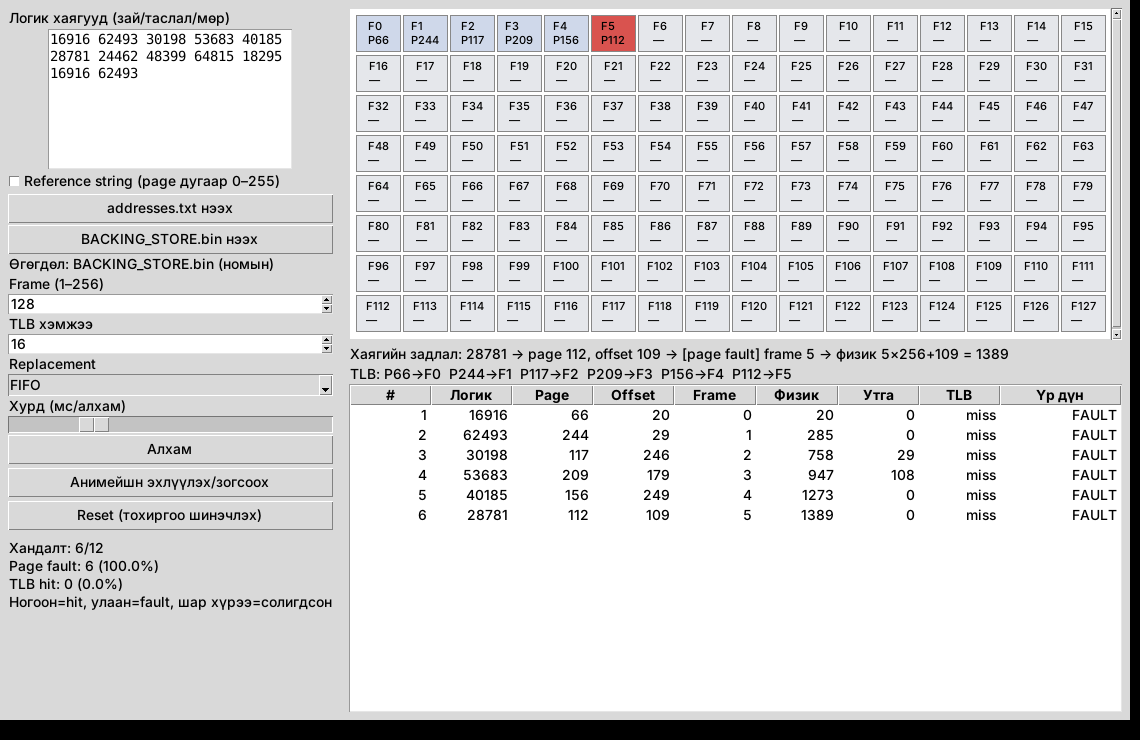
\includegraphics[width=\linewidth]{gui_fault.png}\caption{Анхдагч 12 хаяг, 6 дахь алхам: page fault (улаан)}\end{subfigure}\hfill
\begin{subfigure}[t]{0.49\linewidth}\centering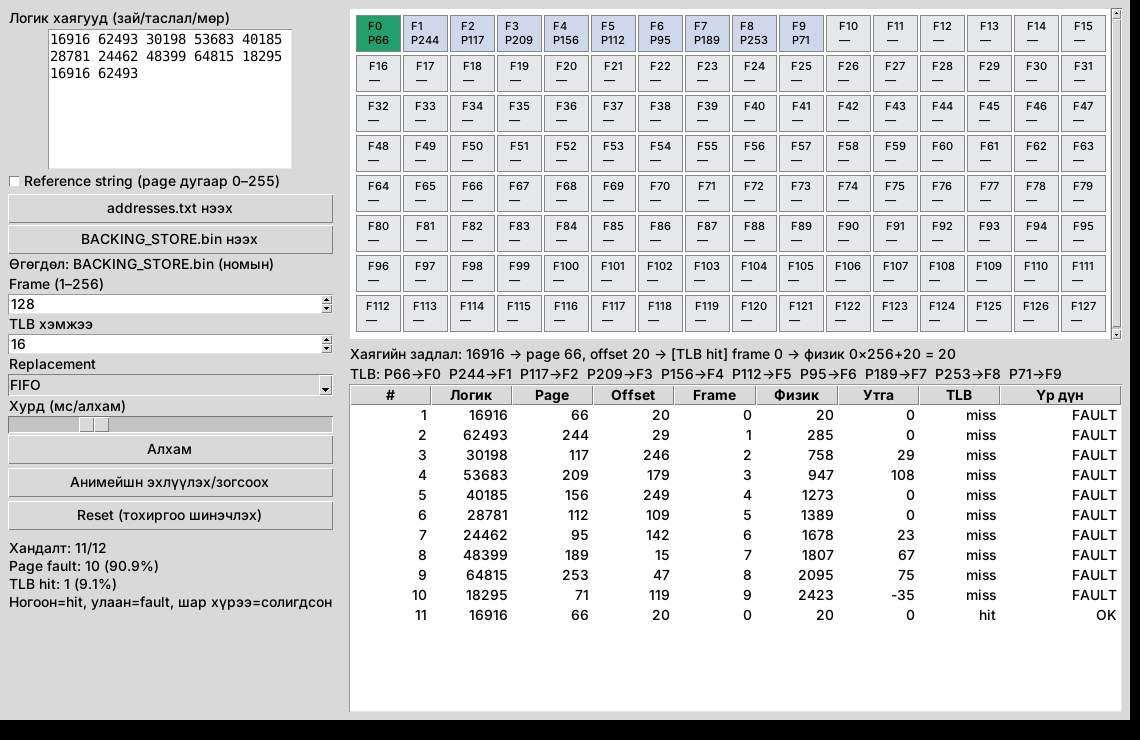
\includegraphics[width=\linewidth]{gui_tlbhit.png}\caption{11 дэх алхам: 16916 дахин ирж TLB hit (ногоон). Утгууд (0, 0, 29, 108, …) \texttt{correct.txt}-тэй таарна}\end{subfigure}\\[6pt]
\begin{subfigure}[t]{0.49\linewidth}\centering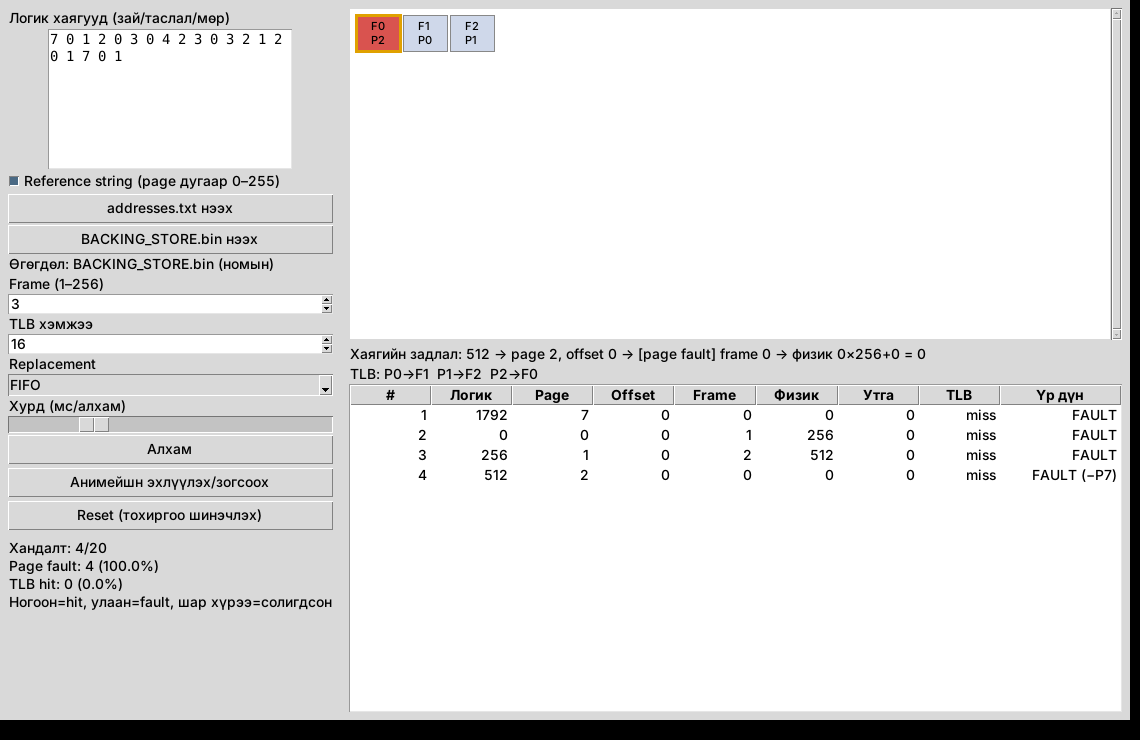
\includegraphics[width=\linewidth]{gui_evict.png}\caption{FIFO, 3 frame: P7-г гаргасан (шар хүрээ, \texttt{FAULT (−P7)})}\end{subfigure}\hfill
\begin{subfigure}[t]{0.49\linewidth}\centering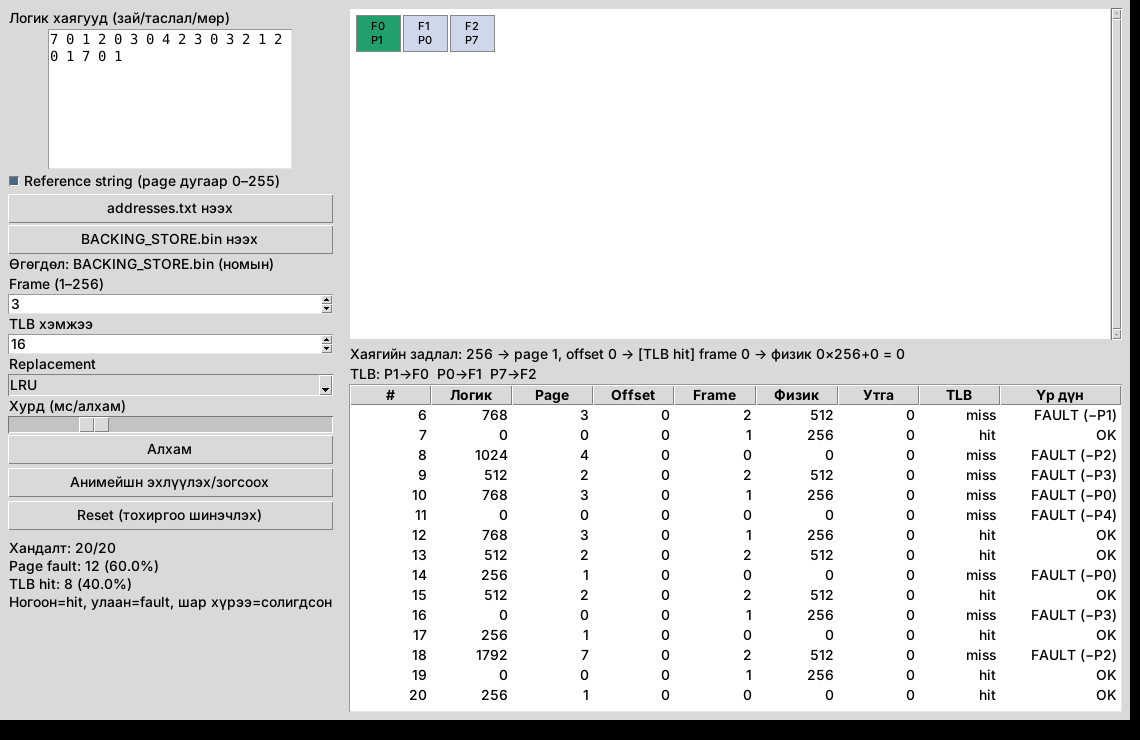
\includegraphics[width=\linewidth]{gui_lru.png}\caption{LRU, 3 frame: 20 хандалтаас 12 fault, номтой таарсан}\end{subfigure}
\caption{GUI-ийн бодит төлөвүүд}\end{figure}
\begin{figure}[H]\centering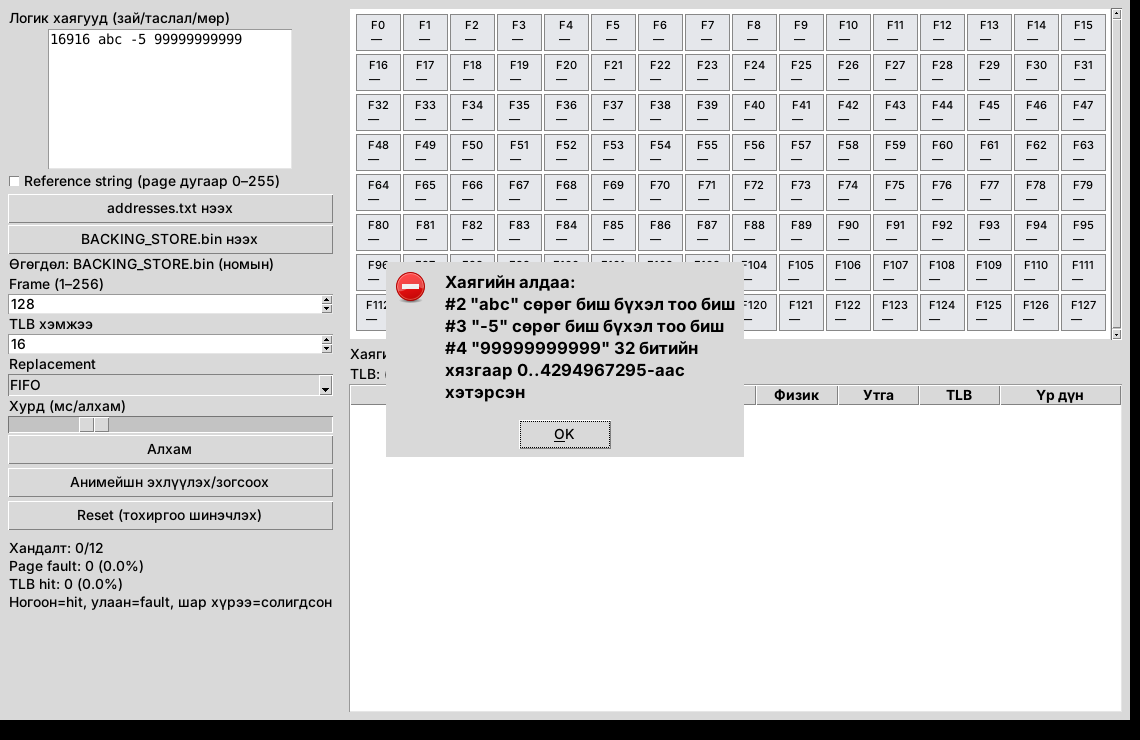
\includegraphics[width=0.6\linewidth]{gui_error.png}
\caption{Алдаатай оролтыг дугаар болон шалтгааны хамт мэдээлж байна}\end{figure}

% ---------------------------------------------------------------
\section{Хэлэлцүүлэг}
\subsection{Үр дүнгийн тайлбар}
\begin{itemize}
\item \textbf{Зөв ажиллагаа.} Номын \texttt{correct.txt}-тэй 1000/1000 мөр таарсан. Энэ нь хаяг задлах, TLB, page table, demand paging, backing store-оос унших, signed byte хөрвүүлэлт бүгд зөв ажиллаж байгааг харуулна. 128 frame-тэй үед ч утга бүгд зөв гарсан нь солилт болон дахин ачаалах логик зөв гэдгийг нотолно. Номын FIFO/LRU жишээ ч тоогоороо таарсан.
\item \textbf{LRU ба FIFO (locality).} Locality-тэй ачаалалд, ажлын олонлог frame-д арай ядан багтах үед LRU илт давуу байв (16 frame-тэй үед 22.6\% vs 27.7\%). Учир нь FIFO байнга хэрэглэгдэж буй „хуучин“ page-ийг гаргадаг. Frame хангалттай олон болоход хоёр бодлого хоёулаа зөвхөн анхны (cold) fault-тай болж ижилсдэг. 256 frame-тэй үед гарсан 161 fault нь өгөгдөл дэх ялгаатай page-ийн тоотой тэнцүү.
\item \textbf{Номын хаяг (санамсаргүй).} Номын хаягууд санамсаргүй үүсгэгдсэн тул locality байхгүй. Ийм үед ирээдүйн хандалтыг өнгөрснөөр таах боломжгүй тул LRU-гийн давуу тал алга болно. 128 frame-тэй үед LRU (539) нь FIFO-оос (538) ч нэгээр илүү fault гаргасан. Fault rate ойролцоогоор $1-\text{frames}/256$ байв (64 frame → 76.2\%). 256 frame-тэй үеийн 244 fault нь \texttt{addresses.txt} дахь ялгаатай page-ийн тоотой яг тэнцүү.
\item \textbf{TLB.} Locality-тэй өгөгдөлд 16 оролттой TLB хандалтын ~3/4-ийг page table руу хандалгүй хөрвүүлсэн. Ажлын олонлог 12 page тул 32-оос том TLB бараг ашиг өгсөнгүй. Харин номын санамсаргүй хаягуудад TLB hit ердөө 5.4\% байв. Ном өөрөө ч эдгээр хаягуудад locality байхгүй тул TLB hit rate өндөр гарахгүй гэж тэмдэглэсэн байдаг.
\item \textbf{Belady.} FIFO нь stack алгоритм биш тул frame нэмэхэд fault өсөж болохыг харууллаа. LRU-д ийм үзэгдэл ажиглагдаагүй.
\end{itemize}
\subsection{Хязгаарлалт ба мэдэгдэж буй асуудлууд}
\begin{itemize}
\item \textbf{Хамрах хүрээ.} Бичих үйлдэл (dirty bit), олон процесс, хоёр түвшний page table хэрэгжээгүй.
\item \textbf{TLB хайлт.} TLB-д шугаман хайлт хийдэг ($O(T)$). Бодит TLB зэрэгцээ (associative) хайдаг тул энэ нь симуляцийн хялбарчлал юм. TLB-ийн бодлогыг page replacement-ээс тусад нь сонгох боломжгүй.
\item \textbf{Locality өгөгдөл.} Өөрсдийн загварчилсан (synthetic) өгөгдөл тул бодит програмын хандалтыг бүрэн төлөөлөхгүй.
\item \textbf{GUI.} tkinter шаардлагатай (Linux дээр \texttt{python3-tk}). Тохиргоо өөрчилсний дараа Reset дарах хэрэгтэй.
\end{itemize}

% ---------------------------------------------------------------
\section{Дүгнэлт}
Сурах бичгийн Programming Project-ийн үндсэн функц бүрэн хэрэгжсэн: хаяг задлах, 16 оролттой TLB, page table, физик санах ой ба demand paging, 1–256 frame-тэй үеийн FIFO ба LRU солилт, номын форматтай гаралт. Програмын зөв ажиллагааг номын албан ёсны \texttt{correct.txt}-ээр баталгаажуулсан: 1000/1000 мөр таарсан. Багшийн шаардсан \textbf{page/frame animation} цөмтэй шууд холбогдсон. Хэрэглэгч хаяг/reference string, frame, TLB, policy-г сольж, алхам эсвэл анимейшнээр ажиглах, reset хийх боломжтой.

Номын жишээтэй таарсан үр дүн (FIFO 15 / LRU 12, Belady 9 → 10) гарсан. Мөн locality-тэй ачаалалд LRU давуу байдаг, санамсаргүй хаягт давуу тал нь алга болдог, TLB 16–32 оролтод ханадаг гэдгийг тоон үр дүнгээр нотоллоо. Буруу болон захын оролтыг ойлгомжтой мэдээлж, 24 автомат тест бүгд амжилттай давсан. Цаашид dirty bit ба write-back, тусдаа TLB бодлого нэмэх, бодит програмын хандалтын trace-ээр турших боломжтой.

% ---------------------------------------------------------------
\section*{Ашигласан материал}\addcontentsline{toc}{section}{Ашигласан материал}
\begin{itemize}
\item A. Silberschatz, P. B. Galvin, G. Gagne. \textit{Operating System Concepts}, 10th ed. Wiley, 2018. Chapter 10, Programming Project „Designing a Virtual Memory Manager“.
\item G. Gagne. \textit{OSC10e source code}, ch10 (\texttt{addresses.txt}, \texttt{BACKING\_STORE.bin}, \texttt{correct.txt}). \href{https://github.com/greggagne/osc10e}{\texttt{github.com/greggagne/osc10e}}
\item L. A. Belady, R. A. Nelson, G. S. Shedler. „An anomaly in space-time characteristics of certain programs running in a paging machine.“ \textit{Communications of the ACM}, 12(6), 1969.
\item Python Software Foundation. \textit{Python 3 documentation}: tkinter, argparse, unittest. \href{https://docs.python.org/3/}{\texttt{docs.python.org/3}}
\item F.CSM302 „Бие даалт 1“ заавар ба „Сэдэв ба шүүмжийн хуваарилалт“, 2026.
\item Төслийн код: \href{https://github.com/ws202-gg/Designing-a-Virtual-Memory-Manager}{\texttt{github.com/ws202-gg/Designing-a-Virtual-Memory-Manager}}
\end{itemize}

\section*{Хавсралт A. Ажлын төлөвлөгөө}\addcontentsline{toc}{section}{Хавсралт A. Ажлын төлөвлөгөө}
\begin{tabularx}{\linewidth}{@{}>{\raggedright\arraybackslash}p{4cm}Y@{}}
\hdr\hc{Талбар}&\hc{Мэдээлэл}\\
\textbf{Хуваарилалтын код}&II-4-15\\
\textbf{Төсөл}&Designing a Virtual Memory Manager (page/frame animation)\\
\textbf{Repository}&\href{https://github.com/ws202-gg/Designing-a-Virtual-Memory-Manager}{\texttt{github.com/ws202-gg/Designing-a-Virtual-Memory-Manager}}\\
\textbf{Хэл/сан/орчин}&Python 3.10+, tkinter, unittest. Linux / Windows / macOS\\
\textbf{Үндсэн дүрслэл}&Page/frame animation (frame grid, TLB, hit / fault / evict өнгө)\\
\end{tabularx}
\vspace{8pt}

\begin{tabularx}{\linewidth}{@{}>{\raggedright\arraybackslash}p{4.1cm}Y>{\raggedright\arraybackslash}p{4.7cm}@{}}
\hdr\hc{Гишүүн}&\hc{Хариуцах ажил}&\hc{Commit / file}\\
Э.Мөнх-Оргил /B242270130/&Багийн ахлагч. VMM цөм (хаяг задлах, TLB, page table, FIFO/LRU)&\texttt{src/vmm.py}\\
Д.Ундармаа /B242270044/&Interactive UI (page/frame animation)&\texttt{src/gui.py}\\
В.Хүсэлбилэг /B241910007/&Консол програм, тайлан (Report)&\texttt{src/cli.py}, \texttt{docs/…Report.pdf}\\
С.Сүхбат /B241940044/&Автомат тест, boundary/error тест, GitHub repository ба Release v1.0&\texttt{tests/}, \texttt{tools/check\_correct.py}, \texttt{README.md}\\
М.Хатансайхан /B231940049/&Туршилтын скрипт, туршилтын өгөгдөл, screenshot, график&\texttt{src/experiment.py}, \texttt{examples/}, \texttt{docs/img/}\\
\end{tabularx}
\vspace{8pt}

\begin{tabularx}{\linewidth}{@{}l>{\raggedright\arraybackslash}p{6.4cm}Y@{}}
\hdr\hc{Тест}&\hc{Оролт/нөхцөл}&\hc{Хүлээгдсэн үр дүн}\\
1&Номын өгөгдөл (\texttt{examples/book/}), 256 frame&\texttt{correct.txt}-тэй 1000/1000 мөр. 244 fault, 54 TLB hit\\
2&Номын өгөгдөл, 128 frame, FIFO / LRU&Утга 1000/1000. 538 / 539 fault\\
3&ref\_textbook, 3 frame, FIFO / LRU&15 / 12 fault\\
4&ref\_belady, FIFO, 3 ба 4 frame&9 ба 10 fault\\
5&boundary.txt&65536 → page 0. Програм унахгүй\\
6&bad\_input.txt, empty.txt&Алдааны мессеж, exit 2\\
7&addresses\_1000\_locality, 16 frame&LRU 22.6\% < FIFO 27.7\%\\
\end{tabularx}

\end{document}
